\documentclass[twoside]{book}

% Packages required by doxygen
\usepackage{fixltx2e}
\usepackage{calc}
\usepackage{doxygen}
\usepackage[export]{adjustbox} % also loads graphicx
\usepackage{graphicx}
\usepackage[utf8]{inputenc}
\usepackage{makeidx}
\usepackage{multicol}
\usepackage{multirow}
\PassOptionsToPackage{warn}{textcomp}
\usepackage{textcomp}
\usepackage[nointegrals]{wasysym}
\usepackage[table]{xcolor}

% Font selection
\usepackage[T1]{fontenc}
\usepackage[scaled=.90]{helvet}
\usepackage{courier}
\usepackage{amssymb}
\usepackage{sectsty}
\renewcommand{\familydefault}{\sfdefault}
\allsectionsfont{%
  \fontseries{bc}\selectfont%
  \color{darkgray}%
}
\renewcommand{\DoxyLabelFont}{%
  \fontseries{bc}\selectfont%
  \color{darkgray}%
}
\newcommand{\+}{\discretionary{\mbox{\scriptsize$\hookleftarrow$}}{}{}}

% Page & text layout
\usepackage{geometry}
\geometry{%
  a4paper,%
  top=2.5cm,%
  bottom=2.5cm,%
  left=2.5cm,%
  right=2.5cm%
}
\tolerance=750
\hfuzz=15pt
\hbadness=750
\setlength{\emergencystretch}{15pt}
\setlength{\parindent}{0cm}
\setlength{\parskip}{3ex plus 2ex minus 2ex}
\makeatletter
\renewcommand{\paragraph}{%
  \@startsection{paragraph}{4}{0ex}{-1.0ex}{1.0ex}{%
    \normalfont\normalsize\bfseries\SS@parafont%
  }%
}
\renewcommand{\subparagraph}{%
  \@startsection{subparagraph}{5}{0ex}{-1.0ex}{1.0ex}{%
    \normalfont\normalsize\bfseries\SS@subparafont%
  }%
}
\makeatother

% Headers & footers
\usepackage{fancyhdr}
\pagestyle{fancyplain}
\fancyhead[LE]{\fancyplain{}{\bfseries\thepage}}
\fancyhead[CE]{\fancyplain{}{}}
\fancyhead[RE]{\fancyplain{}{\bfseries\leftmark}}
\fancyhead[LO]{\fancyplain{}{\bfseries\rightmark}}
\fancyhead[CO]{\fancyplain{}{}}
\fancyhead[RO]{\fancyplain{}{\bfseries\thepage}}
\fancyfoot[LE]{\fancyplain{}{}}
\fancyfoot[CE]{\fancyplain{}{}}
\fancyfoot[RE]{\fancyplain{}{\bfseries\scriptsize Generated by Doxygen }}
\fancyfoot[LO]{\fancyplain{}{\bfseries\scriptsize Generated by Doxygen }}
\fancyfoot[CO]{\fancyplain{}{}}
\fancyfoot[RO]{\fancyplain{}{}}
\renewcommand{\footrulewidth}{0.4pt}
\renewcommand{\chaptermark}[1]{%
  \markboth{#1}{}%
}
\renewcommand{\sectionmark}[1]{%
  \markright{\thesection\ #1}%
}

% Indices & bibliography
\usepackage{natbib}
\usepackage[titles]{tocloft}
\setcounter{tocdepth}{3}
\setcounter{secnumdepth}{5}
\makeindex

% Hyperlinks (required, but should be loaded last)
\usepackage{ifpdf}
\ifpdf
  \usepackage[pdftex,pagebackref=true]{hyperref}
\else
  \usepackage[ps2pdf,pagebackref=true]{hyperref}
\fi
\hypersetup{%
  colorlinks=true,%
  linkcolor=blue,%
  citecolor=blue,%
  unicode%
}

% Custom commands
\newcommand{\clearemptydoublepage}{%
  \newpage{\pagestyle{empty}\cleardoublepage}%
}

\usepackage{caption}
\captionsetup{labelsep=space,justification=centering,font={bf},singlelinecheck=off,skip=4pt,position=top}

%===== C O N T E N T S =====

\begin{document}

% Titlepage & ToC
\hypersetup{pageanchor=false,
             bookmarksnumbered=true,
             pdfencoding=unicode
            }
\pagenumbering{roman}
\begin{titlepage}
\vspace*{7cm}
\begin{center}%
{\Large My Project }\\
\vspace*{1cm}
{\large Generated by Doxygen 1.8.11}\\
\end{center}
\end{titlepage}
\clearemptydoublepage
\tableofcontents
\clearemptydoublepage
\pagenumbering{arabic}
\hypersetup{pageanchor=true}

%--- Begin generated contents ---
\chapter{Class Index}
\section{Class List}
Here are the classes, structs, unions and interfaces with brief descriptions\+:\begin{DoxyCompactList}
\item\contentsline{section}{\hyperlink{classgraph2D}{graph2D} \\*Class for 2D graph }{\pageref{classgraph2D}}{}
\item\contentsline{section}{\hyperlink{classgraph3D}{graph3D} \\*Class for 3D graph }{\pageref{classgraph3D}}{}
\item\contentsline{section}{\hyperlink{classinput__mode}{input\+\_\+mode} \\*User Mode selection is done here }{\pageref{classinput__mode}}{}
\item\contentsline{section}{\hyperlink{classinputfile__to__2D__graphs}{inputfile\+\_\+to\+\_\+2\+D\+\_\+graphs} \\*An input file is converted into 3 2D graphs }{\pageref{classinputfile__to__2D__graphs}}{}
\item\contentsline{section}{\hyperlink{classinputfile__to__3D__graph}{inputfile\+\_\+to\+\_\+3\+D\+\_\+graph} \\*An input file is converted to a 3D graph }{\pageref{classinputfile__to__3D__graph}}{}
\item\contentsline{section}{\hyperlink{classmyvector}{myvector} }{\pageref{classmyvector}}{}
\item\contentsline{section}{\hyperlink{classoutput}{output} \\*The output graphs are converted into a list and these lists are printed in an output file }{\pageref{classoutput}}{}
\item\contentsline{section}{\hyperlink{classplane}{plane} \\*Class for a 3D plane }{\pageref{classplane}}{}
\item\contentsline{section}{\hyperlink{classvertex2D}{vertex2D} \\*Class for representing a 2D labelled vertex The vertex has a label and 2 coordinates }{\pageref{classvertex2D}}{}
\item\contentsline{section}{\hyperlink{classvertex3D}{vertex3D} \\*Class for representing a 3D labelled vertex The vertex has a label and 3 coordinates }{\pageref{classvertex3D}}{}
\end{DoxyCompactList}

\chapter{File Index}
\section{File List}
Here is a list of all files with brief descriptions\+:\begin{DoxyCompactList}
\item\contentsline{section}{\hyperlink{Canvas_8cpp}{Canvas.\+cpp} }{\pageref{Canvas_8cpp}}{}
\item\contentsline{section}{\hyperlink{Input__mode_8cpp}{Input\+\_\+mode.\+cpp} }{\pageref{Input__mode_8cpp}}{}
\item\contentsline{section}{\hyperlink{main_8cpp}{main.\+cpp} }{\pageref{main_8cpp}}{}
\item\contentsline{section}{\hyperlink{main__computation_8cpp}{main\+\_\+computation.\+cpp} }{\pageref{main__computation_8cpp}}{}
\item\contentsline{section}{\hyperlink{Output_8cpp}{Output.\+cpp} }{\pageref{Output_8cpp}}{}
\end{DoxyCompactList}

\chapter{Class Documentation}
\hypertarget{classgraph2D}{}\section{graph2D Class Reference}
\label{classgraph2D}\index{graph2D@{graph2D}}


Class for 2D graph.  


\subsection*{Public Member Functions}
\begin{DoxyCompactItemize}
\item 
\hyperlink{classgraph2D_a4702eac5247e6a9c9336b212b105dddf}{graph2D} (int s)
\begin{DoxyCompactList}\small\item\em A Constructor. \end{DoxyCompactList}\item 
void \hyperlink{classgraph2D_a0bc80a8850d11d49722f30fd0081dc1e}{addvertex} (\hyperlink{classvertex2D}{vertex2D} $\ast$a)
\begin{DoxyCompactList}\small\item\em A Member function which adds the arguement 2D vertex to the graph. \end{DoxyCompactList}\item 
void \hyperlink{classgraph2D_a1ec89f9154f7a06ca9440c54114a5ae8}{addedge} (\hyperlink{classvertex2D}{vertex2D} $\ast$a, \hyperlink{classvertex2D}{vertex2D} $\ast$b, int c)
\begin{DoxyCompactList}\small\item\em A Member function which adds an edge to graph. \end{DoxyCompactList}\item 
int \hyperlink{classgraph2D_a49365267df78a75819ef8a8647a514d0}{indexis} (\hyperlink{classvertex2D}{vertex2D} $\ast$a)
\begin{DoxyCompactList}\small\item\em A Member function which returns the index of the arguement vertex else -\/1. \end{DoxyCompactList}\item 
bool \hyperlink{classgraph2D_a82180cab2d84b3ec314b9941a600227c}{isvertex} (\hyperlink{classvertex2D}{vertex2D} $\ast$a)
\begin{DoxyCompactList}\small\item\em A Member function which tells if a vertex is in the graph or not. \end{DoxyCompactList}\item 
bool \hyperlink{classgraph2D_a81175519185c21347127968da495ce75}{isedge} (\hyperlink{classvertex2D}{vertex2D} $\ast$a, \hyperlink{classvertex2D}{vertex2D} $\ast$b)
\begin{DoxyCompactList}\small\item\em A Member function which tells if an edge is in the graph or not. \end{DoxyCompactList}\item 
void \hyperlink{classgraph2D_a060f2ba8f4edbd896fafe5d4e7990b86}{make\+\_\+2\+Dgraph\+\_\+with\+\_\+vertices} (\hyperlink{classgraph3D}{graph3D} g, \hyperlink{classplane}{plane} p)
\begin{DoxyCompactList}\small\item\em A Member function which adds the 2D graph(only vertices) corresponding to a given 3D graph and a projection plane. \end{DoxyCompactList}\item 
void \hyperlink{classgraph2D_ae7f6f12a73326f7cbbaa3f87ea59c0ad}{join\+\_\+2\+D\+\_\+edges} (\hyperlink{classgraph3D}{graph3D} g)
\begin{DoxyCompactList}\small\item\em A Member function which adds the corresponding edges in 2D graph(which has the projected vertices) w.\+r.\+t to a given 3D graph. \end{DoxyCompactList}\item 
void \hyperlink{classgraph2D_a713850a586c412115558b9c34e0bef5a}{filter\+\_\+hidden\+\_\+lines} (\hyperlink{classgraph3D}{graph3D} g, \hyperlink{classplane}{plane} p)
\begin{DoxyCompactList}\small\item\em A Member function filters hidden lines from the 2D graph. \end{DoxyCompactList}\end{DoxyCompactItemize}


\subsection{Detailed Description}
Class for 2D graph. 

\begin{DoxySeeAlso}{See also}
\hyperlink{classvertex2D}{vertex2D} 
\end{DoxySeeAlso}


\subsection{Constructor \& Destructor Documentation}
\index{graph2D@{graph2D}!graph2D@{graph2D}}
\index{graph2D@{graph2D}!graph2D@{graph2D}}
\subsubsection[{\texorpdfstring{graph2\+D(int s)}{graph2D(int s)}}]{\setlength{\rightskip}{0pt plus 5cm}graph2\+D\+::graph2D (
\begin{DoxyParamCaption}
\item[{int}]{s}
\end{DoxyParamCaption}
)}\hypertarget{classgraph2D_a4702eac5247e6a9c9336b212b105dddf}{}\label{classgraph2D_a4702eac5247e6a9c9336b212b105dddf}


A Constructor. 

The constructor constructs the graph with one arguement\+: an integer which is the size of graph. 
\begin{DoxyParams}{Parameters}
{\em s} & the number of vertices. \\
\hline
\end{DoxyParams}


\subsection{Member Function Documentation}
\index{graph2D@{graph2D}!addedge@{addedge}}
\index{addedge@{addedge}!graph2D@{graph2D}}
\subsubsection[{\texorpdfstring{addedge(vertex2\+D $\ast$a, vertex2\+D $\ast$b, int c)}{addedge(vertex2D *a, vertex2D *b, int c)}}]{\setlength{\rightskip}{0pt plus 5cm}void graph2\+D\+::addedge (
\begin{DoxyParamCaption}
\item[{{\bf vertex2D} $\ast$}]{a, }
\item[{{\bf vertex2D} $\ast$}]{b, }
\item[{int}]{c}
\end{DoxyParamCaption}
)}\hypertarget{classgraph2D_a1ec89f9154f7a06ca9440c54114a5ae8}{}\label{classgraph2D_a1ec89f9154f7a06ca9440c54114a5ae8}


A Member function which adds an edge to graph. 


\begin{DoxyParams}{Parameters}
{\em a} & The end vertex of the edge to be added. \\
\hline
{\em b} & The other end vertex of the edge to be added. \\
\hline
{\em c} & An integer which is either 1(normal edge) or 2(hidden edge) or 0(no edge). \\
\hline
\end{DoxyParams}
\index{graph2D@{graph2D}!addvertex@{addvertex}}
\index{addvertex@{addvertex}!graph2D@{graph2D}}
\subsubsection[{\texorpdfstring{addvertex(vertex2\+D $\ast$a)}{addvertex(vertex2D *a)}}]{\setlength{\rightskip}{0pt plus 5cm}void graph2\+D\+::addvertex (
\begin{DoxyParamCaption}
\item[{{\bf vertex2D} $\ast$}]{a}
\end{DoxyParamCaption}
)}\hypertarget{classgraph2D_a0bc80a8850d11d49722f30fd0081dc1e}{}\label{classgraph2D_a0bc80a8850d11d49722f30fd0081dc1e}


A Member function which adds the arguement 2D vertex to the graph. 


\begin{DoxyParams}{Parameters}
{\em a} & The 2D vertex to be added. \\
\hline
\end{DoxyParams}
\index{graph2D@{graph2D}!filter\+\_\+hidden\+\_\+lines@{filter\+\_\+hidden\+\_\+lines}}
\index{filter\+\_\+hidden\+\_\+lines@{filter\+\_\+hidden\+\_\+lines}!graph2D@{graph2D}}
\subsubsection[{\texorpdfstring{filter\+\_\+hidden\+\_\+lines(graph3\+D g, plane p)}{filter_hidden_lines(graph3D g, plane p)}}]{\setlength{\rightskip}{0pt plus 5cm}void graph2\+D\+::filter\+\_\+hidden\+\_\+lines (
\begin{DoxyParamCaption}
\item[{{\bf graph3D}}]{g, }
\item[{{\bf plane}}]{p}
\end{DoxyParamCaption}
)}\hypertarget{classgraph2D_a713850a586c412115558b9c34e0bef5a}{}\label{classgraph2D_a713850a586c412115558b9c34e0bef5a}


A Member function filters hidden lines from the 2D graph. 

This function will always be called after calling the make\+\_\+2\+D\+\_\+graph\+\_\+with\+\_\+vertices and join\+\_\+2\+D\+\_\+edges function. Here, first we convert the 2D coordinates of 2D graph into 3D vertex, then we see if the projected 3\+Dvertex and 3\+Dvertex are on same side of any face in face set. If yes, then edges from the vertex are done hidden. 
\begin{DoxyParams}{Parameters}
{\em g} & The 3D graph which contains the set of faces. \\
\hline
{\em p} & The projected plane \\
\hline
\end{DoxyParams}
\begin{DoxySeeAlso}{See also}
\hyperlink{classgraph2D_ae7f6f12a73326f7cbbaa3f87ea59c0ad}{join\+\_\+2\+D\+\_\+edges()} 

\hyperlink{classgraph2D_a060f2ba8f4edbd896fafe5d4e7990b86}{make\+\_\+2\+Dgraph\+\_\+with\+\_\+vertices()} 
\end{DoxySeeAlso}
\index{graph2D@{graph2D}!indexis@{indexis}}
\index{indexis@{indexis}!graph2D@{graph2D}}
\subsubsection[{\texorpdfstring{indexis(vertex2\+D $\ast$a)}{indexis(vertex2D *a)}}]{\setlength{\rightskip}{0pt plus 5cm}int graph2\+D\+::indexis (
\begin{DoxyParamCaption}
\item[{{\bf vertex2D} $\ast$}]{a}
\end{DoxyParamCaption}
)}\hypertarget{classgraph2D_a49365267df78a75819ef8a8647a514d0}{}\label{classgraph2D_a49365267df78a75819ef8a8647a514d0}


A Member function which returns the index of the arguement vertex else -\/1. 


\begin{DoxyParams}{Parameters}
{\em a} & The 2D vertex. \\
\hline
\end{DoxyParams}
\begin{DoxyReturn}{Returns}
The index. 
\end{DoxyReturn}
\index{graph2D@{graph2D}!isedge@{isedge}}
\index{isedge@{isedge}!graph2D@{graph2D}}
\subsubsection[{\texorpdfstring{isedge(vertex2\+D $\ast$a, vertex2\+D $\ast$b)}{isedge(vertex2D *a, vertex2D *b)}}]{\setlength{\rightskip}{0pt plus 5cm}bool graph2\+D\+::isedge (
\begin{DoxyParamCaption}
\item[{{\bf vertex2D} $\ast$}]{a, }
\item[{{\bf vertex2D} $\ast$}]{b}
\end{DoxyParamCaption}
)}\hypertarget{classgraph2D_a81175519185c21347127968da495ce75}{}\label{classgraph2D_a81175519185c21347127968da495ce75}


A Member function which tells if an edge is in the graph or not. 


\begin{DoxyParams}{Parameters}
{\em a} & One end of the edge to be checked. \\
\hline
{\em b} & Other end of the edge to be checked. \\
\hline
\end{DoxyParams}
\begin{DoxyReturn}{Returns}
boolean type variable. 
\end{DoxyReturn}
\index{graph2D@{graph2D}!isvertex@{isvertex}}
\index{isvertex@{isvertex}!graph2D@{graph2D}}
\subsubsection[{\texorpdfstring{isvertex(vertex2\+D $\ast$a)}{isvertex(vertex2D *a)}}]{\setlength{\rightskip}{0pt plus 5cm}bool graph2\+D\+::isvertex (
\begin{DoxyParamCaption}
\item[{{\bf vertex2D} $\ast$}]{a}
\end{DoxyParamCaption}
)}\hypertarget{classgraph2D_a82180cab2d84b3ec314b9941a600227c}{}\label{classgraph2D_a82180cab2d84b3ec314b9941a600227c}


A Member function which tells if a vertex is in the graph or not. 


\begin{DoxyParams}{Parameters}
{\em a} & The 2D vertex to be checked. \\
\hline
\end{DoxyParams}
\begin{DoxyReturn}{Returns}
boolean type variable. 
\end{DoxyReturn}
\index{graph2D@{graph2D}!join\+\_\+2\+D\+\_\+edges@{join\+\_\+2\+D\+\_\+edges}}
\index{join\+\_\+2\+D\+\_\+edges@{join\+\_\+2\+D\+\_\+edges}!graph2D@{graph2D}}
\subsubsection[{\texorpdfstring{join\+\_\+2\+D\+\_\+edges(graph3\+D g)}{join_2D_edges(graph3D g)}}]{\setlength{\rightskip}{0pt plus 5cm}void graph2\+D\+::join\+\_\+2\+D\+\_\+edges (
\begin{DoxyParamCaption}
\item[{{\bf graph3D}}]{g}
\end{DoxyParamCaption}
)}\hypertarget{classgraph2D_ae7f6f12a73326f7cbbaa3f87ea59c0ad}{}\label{classgraph2D_ae7f6f12a73326f7cbbaa3f87ea59c0ad}


A Member function which adds the corresponding edges in 2D graph(which has the projected vertices) w.\+r.\+t to a given 3D graph. 

This function will always be called after calling the make\+\_\+2\+D\+\_\+graph\+\_\+with\+\_\+vertices function. 
\begin{DoxyParams}{Parameters}
{\em g} & The 3D graph though which edge are to be projected. \\
\hline
\end{DoxyParams}
\begin{DoxySeeAlso}{See also}
\hyperlink{classgraph2D_a060f2ba8f4edbd896fafe5d4e7990b86}{make\+\_\+2\+Dgraph\+\_\+with\+\_\+vertices()} 
\end{DoxySeeAlso}
\index{graph2D@{graph2D}!make\+\_\+2\+Dgraph\+\_\+with\+\_\+vertices@{make\+\_\+2\+Dgraph\+\_\+with\+\_\+vertices}}
\index{make\+\_\+2\+Dgraph\+\_\+with\+\_\+vertices@{make\+\_\+2\+Dgraph\+\_\+with\+\_\+vertices}!graph2D@{graph2D}}
\subsubsection[{\texorpdfstring{make\+\_\+2\+Dgraph\+\_\+with\+\_\+vertices(graph3\+D g, plane p)}{make_2Dgraph_with_vertices(graph3D g, plane p)}}]{\setlength{\rightskip}{0pt plus 5cm}void graph2\+D\+::make\+\_\+2\+Dgraph\+\_\+with\+\_\+vertices (
\begin{DoxyParamCaption}
\item[{{\bf graph3D}}]{g, }
\item[{{\bf plane}}]{p}
\end{DoxyParamCaption}
)}\hypertarget{classgraph2D_a060f2ba8f4edbd896fafe5d4e7990b86}{}\label{classgraph2D_a060f2ba8f4edbd896fafe5d4e7990b86}


A Member function which adds the 2D graph(only vertices) corresponding to a given 3D graph and a projection plane. 

Here we have taken the point(rp) in the plane as origin, so we get a 2D graph with asix (e1) and (e2). 
\begin{DoxyParams}{Parameters}
{\em g} & The 3D graph to be projected. \\
\hline
{\em p} & The plane on which it is to be projected. \\
\hline
\end{DoxyParams}
\begin{DoxySeeAlso}{See also}
\hyperlink{classplane}{plane} 

\hyperlink{classvertex3D}{vertex3D} 
\end{DoxySeeAlso}


The documentation for this class was generated from the following file\+:\begin{DoxyCompactItemize}
\item 
\hyperlink{main__computation_8cpp}{main\+\_\+computation.\+cpp}\end{DoxyCompactItemize}

\hypertarget{classgraph3D}{}\section{graph3D Class Reference}
\label{classgraph3D}\index{graph3D@{graph3D}}


Class for 3D graph.  




Collaboration diagram for graph3D\+:\nopagebreak
\begin{figure}[H]
\begin{center}
\leavevmode
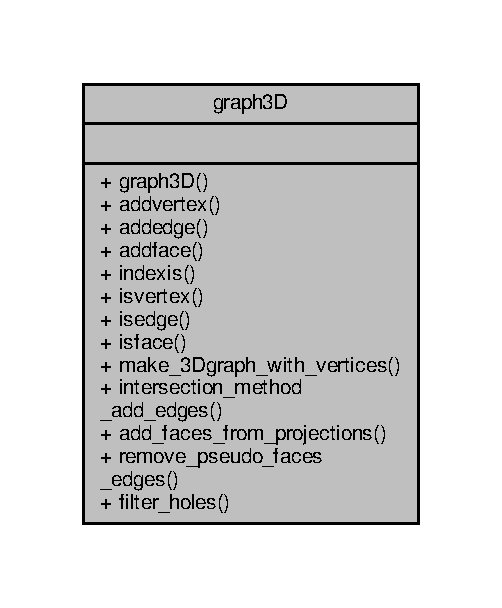
\includegraphics[width=241pt]{classgraph3D__coll__graph}
\end{center}
\end{figure}
\subsection*{Public Member Functions}
\begin{DoxyCompactItemize}
\item 
\hyperlink{classgraph3D_afc08df517e186ff3e3b9e7a7e1f34f44}{graph3D} (int s)
\begin{DoxyCompactList}\small\item\em A Constructor. \end{DoxyCompactList}\item 
void \hyperlink{classgraph3D_afc9caffb42c40e6f952b07295094ad57}{addvertex} (\hyperlink{classvertex3D}{vertex3D} $\ast$a)
\begin{DoxyCompactList}\small\item\em A Member function which adds the arguement 3D vertex to the graph. \end{DoxyCompactList}\item 
void \hyperlink{classgraph3D_a4f2a5e18655c4667438af55a136f381e}{addedge} (\hyperlink{classvertex3D}{vertex3D} $\ast$a, \hyperlink{classvertex3D}{vertex3D} $\ast$b, int c)
\begin{DoxyCompactList}\small\item\em A Member function which adds an edge to graph. \end{DoxyCompactList}\item 
void \hyperlink{classgraph3D_ac2d0f130cd68efe98855a21c9d253159}{addface} (std\+::vector$<$ \hyperlink{classvertex3D}{vertex3D} $\ast$ $>$ v)
\begin{DoxyCompactList}\small\item\em A Member function which adds a face to graph. \end{DoxyCompactList}\item 
int \hyperlink{classgraph3D_ae71fa4ac2b1ea51db4899ee0a57dd59c}{indexis} (\hyperlink{classvertex3D}{vertex3D} $\ast$a)
\begin{DoxyCompactList}\small\item\em A Member function which returns the index of the arguement vertex else -\/1. \end{DoxyCompactList}\item 
bool \hyperlink{classgraph3D_a9d9e7f67e635b5aa896275072b39fbdd}{isvertex} (\hyperlink{classvertex3D}{vertex3D} $\ast$a)
\begin{DoxyCompactList}\small\item\em A Member function which tells if a vertex is in the graph or not. \end{DoxyCompactList}\item 
bool \hyperlink{classgraph3D_ac73a37d6b631a9ae96ab6822cf73c11f}{isedge} (\hyperlink{classvertex3D}{vertex3D} $\ast$a, \hyperlink{classvertex3D}{vertex3D} $\ast$b)
\begin{DoxyCompactList}\small\item\em A Member function which tells if an edge is in the graph or not. \end{DoxyCompactList}\item 
bool \hyperlink{classgraph3D_a30171eb80bcfeb866667964dcaf8f8a6}{isface} (std\+::vector$<$ \hyperlink{classvertex3D}{vertex3D} $\ast$ $>$ v)
\begin{DoxyCompactList}\small\item\em A Member function which tells if a face is in the graph or not. \end{DoxyCompactList}\item 
void \hyperlink{classgraph3D_aa9c7ef09439ee3f7433f80f1ec4798ba}{make\+\_\+3\+Dgraph\+\_\+with\+\_\+vertices} (\hyperlink{classgraph2D}{graph2D} o1, \hyperlink{classgraph2D}{graph2D} o2, \hyperlink{classgraph2D}{graph2D} o3)
\begin{DoxyCompactList}\small\item\em A Member function which adds the 3D graph(only vertices) corresponding to a given set of three orthographic views (2D graph). \end{DoxyCompactList}\item 
void \hyperlink{classgraph3D_a4d45444d8a38ab79394a2e84b0b2e692}{intersection\+\_\+method\+\_\+add\+\_\+edges} (\hyperlink{classgraph2D}{graph2D} o1, \hyperlink{classgraph2D}{graph2D} o2, \hyperlink{classgraph2D}{graph2D} o3)
\begin{DoxyCompactList}\small\item\em A Member function which adds superset of edges to the 3D graph corresponding to a given set of three orthographic views (2D graph) by finding common edges. \end{DoxyCompactList}\item 
void \hyperlink{classgraph3D_aa79b2b133574a9ae324bc14f0d48fc02}{add\+\_\+faces\+\_\+from\+\_\+projections} ()
\begin{DoxyCompactList}\small\item\em A Member function which adds superset of faces to the 3D graph from given edges, using minimum angle searching method. \end{DoxyCompactList}\item 
void \hyperlink{classgraph3D_aab83b82e5b746bd6c380d82b24f09de5}{remove\+\_\+pseudo\+\_\+faces\+\_\+edges} ()
\begin{DoxyCompactList}\small\item\em A Member function which detects and removes the pseudo faces and edges, using the decision making rules. \end{DoxyCompactList}\item 
void \hyperlink{classgraph3D_a551208f9e31233bfd59c631b64007d02}{filter\+\_\+holes} ()
\begin{DoxyCompactList}\small\item\em A Member function which detects and removes the holes from the remaining faces using odd even rule. \end{DoxyCompactList}\end{DoxyCompactItemize}


\subsection{Detailed Description}
Class for 3D graph. 

\begin{DoxySeeAlso}{See also}
\hyperlink{classvertex3D}{vertex3D} 
\end{DoxySeeAlso}


\subsection{Constructor \& Destructor Documentation}
\index{graph3D@{graph3D}!graph3D@{graph3D}}
\index{graph3D@{graph3D}!graph3D@{graph3D}}
\subsubsection[{\texorpdfstring{graph3\+D(int s)}{graph3D(int s)}}]{\setlength{\rightskip}{0pt plus 5cm}graph3\+D\+::graph3D (
\begin{DoxyParamCaption}
\item[{int}]{s}
\end{DoxyParamCaption}
)}\hypertarget{classgraph3D_afc08df517e186ff3e3b9e7a7e1f34f44}{}\label{classgraph3D_afc08df517e186ff3e3b9e7a7e1f34f44}


A Constructor. 

The constructor constructs the graph with one arguement\+: an integer which is the size of graph. 
\begin{DoxyParams}{Parameters}
{\em s} & the number of vertices. \\
\hline
\end{DoxyParams}


\subsection{Member Function Documentation}
\index{graph3D@{graph3D}!add\+\_\+faces\+\_\+from\+\_\+projections@{add\+\_\+faces\+\_\+from\+\_\+projections}}
\index{add\+\_\+faces\+\_\+from\+\_\+projections@{add\+\_\+faces\+\_\+from\+\_\+projections}!graph3D@{graph3D}}
\subsubsection[{\texorpdfstring{add\+\_\+faces\+\_\+from\+\_\+projections()}{add_faces_from_projections()}}]{\setlength{\rightskip}{0pt plus 5cm}void graph3\+D\+::add\+\_\+faces\+\_\+from\+\_\+projections (
\begin{DoxyParamCaption}
{}
\end{DoxyParamCaption}
)}\hypertarget{classgraph3D_aa79b2b133574a9ae324bc14f0d48fc02}{}\label{classgraph3D_aa79b2b133574a9ae324bc14f0d48fc02}


A Member function which adds superset of faces to the 3D graph from given edges, using minimum angle searching method. 

This function will always be called after calling the intersection\+\_\+method\+\_\+add\+\_\+edges function. No parameters needed. \index{graph3D@{graph3D}!addedge@{addedge}}
\index{addedge@{addedge}!graph3D@{graph3D}}
\subsubsection[{\texorpdfstring{addedge(vertex3\+D $\ast$a, vertex3\+D $\ast$b, int c)}{addedge(vertex3D *a, vertex3D *b, int c)}}]{\setlength{\rightskip}{0pt plus 5cm}void graph3\+D\+::addedge (
\begin{DoxyParamCaption}
\item[{{\bf vertex3D} $\ast$}]{a, }
\item[{{\bf vertex3D} $\ast$}]{b, }
\item[{int}]{c}
\end{DoxyParamCaption}
)}\hypertarget{classgraph3D_a4f2a5e18655c4667438af55a136f381e}{}\label{classgraph3D_a4f2a5e18655c4667438af55a136f381e}


A Member function which adds an edge to graph. 


\begin{DoxyParams}{Parameters}
{\em a} & The end vertex of the edge to be added. \\
\hline
{\em b} & The other end vertex of the edge to be added. \\
\hline
{\em c} & An integer which is either 1(normal edge) or 0(no edge). \\
\hline
\end{DoxyParams}
\index{graph3D@{graph3D}!addface@{addface}}
\index{addface@{addface}!graph3D@{graph3D}}
\subsubsection[{\texorpdfstring{addface(std\+::vector$<$ vertex3\+D $\ast$ $>$ v)}{addface(std::vector< vertex3D * > v)}}]{\setlength{\rightskip}{0pt plus 5cm}void graph3\+D\+::addface (
\begin{DoxyParamCaption}
\item[{std\+::vector$<$ {\bf vertex3D} $\ast$ $>$}]{v}
\end{DoxyParamCaption}
)}\hypertarget{classgraph3D_ac2d0f130cd68efe98855a21c9d253159}{}\label{classgraph3D_ac2d0f130cd68efe98855a21c9d253159}


A Member function which adds a face to graph. 

the vercor of 3D vertices is added to faces set of graph. 
\begin{DoxyParams}{Parameters}
{\em v} & The face to be added. \\
\hline
\end{DoxyParams}
\index{graph3D@{graph3D}!addvertex@{addvertex}}
\index{addvertex@{addvertex}!graph3D@{graph3D}}
\subsubsection[{\texorpdfstring{addvertex(vertex3\+D $\ast$a)}{addvertex(vertex3D *a)}}]{\setlength{\rightskip}{0pt plus 5cm}void graph3\+D\+::addvertex (
\begin{DoxyParamCaption}
\item[{{\bf vertex3D} $\ast$}]{a}
\end{DoxyParamCaption}
)}\hypertarget{classgraph3D_afc9caffb42c40e6f952b07295094ad57}{}\label{classgraph3D_afc9caffb42c40e6f952b07295094ad57}


A Member function which adds the arguement 3D vertex to the graph. 


\begin{DoxyParams}{Parameters}
{\em a} & The 3D vertex to be added. \\
\hline
\end{DoxyParams}
\index{graph3D@{graph3D}!filter\+\_\+holes@{filter\+\_\+holes}}
\index{filter\+\_\+holes@{filter\+\_\+holes}!graph3D@{graph3D}}
\subsubsection[{\texorpdfstring{filter\+\_\+holes()}{filter_holes()}}]{\setlength{\rightskip}{0pt plus 5cm}void graph3\+D\+::filter\+\_\+holes (
\begin{DoxyParamCaption}
{}
\end{DoxyParamCaption}
)}\hypertarget{classgraph3D_a551208f9e31233bfd59c631b64007d02}{}\label{classgraph3D_a551208f9e31233bfd59c631b64007d02}


A Member function which detects and removes the holes from the remaining faces using odd even rule. 

This function will always be called after calling the remove\+\_\+pseudo\+\_\+faces\+\_\+edges function. No parameters needed \index{graph3D@{graph3D}!indexis@{indexis}}
\index{indexis@{indexis}!graph3D@{graph3D}}
\subsubsection[{\texorpdfstring{indexis(vertex3\+D $\ast$a)}{indexis(vertex3D *a)}}]{\setlength{\rightskip}{0pt plus 5cm}int graph3\+D\+::indexis (
\begin{DoxyParamCaption}
\item[{{\bf vertex3D} $\ast$}]{a}
\end{DoxyParamCaption}
)}\hypertarget{classgraph3D_ae71fa4ac2b1ea51db4899ee0a57dd59c}{}\label{classgraph3D_ae71fa4ac2b1ea51db4899ee0a57dd59c}


A Member function which returns the index of the arguement vertex else -\/1. 


\begin{DoxyParams}{Parameters}
{\em a} & The 3D vertex. \\
\hline
\end{DoxyParams}
\begin{DoxyReturn}{Returns}
The index. 
\end{DoxyReturn}
\index{graph3D@{graph3D}!intersection\+\_\+method\+\_\+add\+\_\+edges@{intersection\+\_\+method\+\_\+add\+\_\+edges}}
\index{intersection\+\_\+method\+\_\+add\+\_\+edges@{intersection\+\_\+method\+\_\+add\+\_\+edges}!graph3D@{graph3D}}
\subsubsection[{\texorpdfstring{intersection\+\_\+method\+\_\+add\+\_\+edges(graph2\+D o1, graph2\+D o2, graph2\+D o3)}{intersection_method_add_edges(graph2D o1, graph2D o2, graph2D o3)}}]{\setlength{\rightskip}{0pt plus 5cm}void graph3\+D\+::intersection\+\_\+method\+\_\+add\+\_\+edges (
\begin{DoxyParamCaption}
\item[{{\bf graph2D}}]{o1, }
\item[{{\bf graph2D}}]{o2, }
\item[{{\bf graph2D}}]{o3}
\end{DoxyParamCaption}
)}\hypertarget{classgraph3D_a4d45444d8a38ab79394a2e84b0b2e692}{}\label{classgraph3D_a4d45444d8a38ab79394a2e84b0b2e692}


A Member function which adds superset of edges to the 3D graph corresponding to a given set of three orthographic views (2D graph) by finding common edges. 

This function will always be called after calling the make\+\_\+3\+D\+\_\+graph\+\_\+with\+\_\+vertices function. 
\begin{DoxyParams}{Parameters}
{\em o1} & The front view 2D graph. \\
\hline
{\em o2} & The top view 2D graph. \\
\hline
{\em o3} & The top view 2D graph. \\
\hline
\end{DoxyParams}
\begin{DoxySeeAlso}{See also}
\hyperlink{classgraph2D}{graph2D} 
\end{DoxySeeAlso}
\index{graph3D@{graph3D}!isedge@{isedge}}
\index{isedge@{isedge}!graph3D@{graph3D}}
\subsubsection[{\texorpdfstring{isedge(vertex3\+D $\ast$a, vertex3\+D $\ast$b)}{isedge(vertex3D *a, vertex3D *b)}}]{\setlength{\rightskip}{0pt plus 5cm}bool graph3\+D\+::isedge (
\begin{DoxyParamCaption}
\item[{{\bf vertex3D} $\ast$}]{a, }
\item[{{\bf vertex3D} $\ast$}]{b}
\end{DoxyParamCaption}
)}\hypertarget{classgraph3D_ac73a37d6b631a9ae96ab6822cf73c11f}{}\label{classgraph3D_ac73a37d6b631a9ae96ab6822cf73c11f}


A Member function which tells if an edge is in the graph or not. 


\begin{DoxyParams}{Parameters}
{\em a} & One end of the edge to be checked. \\
\hline
{\em b} & Other end of the edge to be checked. \\
\hline
\end{DoxyParams}
\begin{DoxyReturn}{Returns}
boolean type variable. 
\end{DoxyReturn}
\index{graph3D@{graph3D}!isface@{isface}}
\index{isface@{isface}!graph3D@{graph3D}}
\subsubsection[{\texorpdfstring{isface(std\+::vector$<$ vertex3\+D $\ast$ $>$ v)}{isface(std::vector< vertex3D * > v)}}]{\setlength{\rightskip}{0pt plus 5cm}bool graph3\+D\+::isface (
\begin{DoxyParamCaption}
\item[{std\+::vector$<$ {\bf vertex3D} $\ast$ $>$}]{v}
\end{DoxyParamCaption}
)}\hypertarget{classgraph3D_a30171eb80bcfeb866667964dcaf8f8a6}{}\label{classgraph3D_a30171eb80bcfeb866667964dcaf8f8a6}


A Member function which tells if a face is in the graph or not. 


\begin{DoxyParams}{Parameters}
{\em v} & The face to be checked. \\
\hline
\end{DoxyParams}
\begin{DoxyReturn}{Returns}
boolean type variable. 
\end{DoxyReturn}
\index{graph3D@{graph3D}!isvertex@{isvertex}}
\index{isvertex@{isvertex}!graph3D@{graph3D}}
\subsubsection[{\texorpdfstring{isvertex(vertex3\+D $\ast$a)}{isvertex(vertex3D *a)}}]{\setlength{\rightskip}{0pt plus 5cm}bool graph3\+D\+::isvertex (
\begin{DoxyParamCaption}
\item[{{\bf vertex3D} $\ast$}]{a}
\end{DoxyParamCaption}
)}\hypertarget{classgraph3D_a9d9e7f67e635b5aa896275072b39fbdd}{}\label{classgraph3D_a9d9e7f67e635b5aa896275072b39fbdd}


A Member function which tells if a vertex is in the graph or not. 


\begin{DoxyParams}{Parameters}
{\em a} & The 3D vertex to be checked. \\
\hline
\end{DoxyParams}
\begin{DoxyReturn}{Returns}
boolean type variable. 
\end{DoxyReturn}
\index{graph3D@{graph3D}!make\+\_\+3\+Dgraph\+\_\+with\+\_\+vertices@{make\+\_\+3\+Dgraph\+\_\+with\+\_\+vertices}}
\index{make\+\_\+3\+Dgraph\+\_\+with\+\_\+vertices@{make\+\_\+3\+Dgraph\+\_\+with\+\_\+vertices}!graph3D@{graph3D}}
\subsubsection[{\texorpdfstring{make\+\_\+3\+Dgraph\+\_\+with\+\_\+vertices(graph2\+D o1, graph2\+D o2, graph2\+D o3)}{make_3Dgraph_with_vertices(graph2D o1, graph2D o2, graph2D o3)}}]{\setlength{\rightskip}{0pt plus 5cm}void graph3\+D\+::make\+\_\+3\+Dgraph\+\_\+with\+\_\+vertices (
\begin{DoxyParamCaption}
\item[{{\bf graph2D}}]{o1, }
\item[{{\bf graph2D}}]{o2, }
\item[{{\bf graph2D}}]{o3}
\end{DoxyParamCaption}
)}\hypertarget{classgraph3D_aa9c7ef09439ee3f7433f80f1ec4798ba}{}\label{classgraph3D_aa9c7ef09439ee3f7433f80f1ec4798ba}


A Member function which adds the 3D graph(only vertices) corresponding to a given set of three orthographic views (2D graph). 


\begin{DoxyParams}{Parameters}
{\em o1} & The front view 2D graph. \\
\hline
{\em o2} & The top view 2D graph. \\
\hline
{\em o3} & The top view 2D graph. \\
\hline
\end{DoxyParams}
\begin{DoxySeeAlso}{See also}
\hyperlink{classgraph2D}{graph2D} 
\end{DoxySeeAlso}
\index{graph3D@{graph3D}!remove\+\_\+pseudo\+\_\+faces\+\_\+edges@{remove\+\_\+pseudo\+\_\+faces\+\_\+edges}}
\index{remove\+\_\+pseudo\+\_\+faces\+\_\+edges@{remove\+\_\+pseudo\+\_\+faces\+\_\+edges}!graph3D@{graph3D}}
\subsubsection[{\texorpdfstring{remove\+\_\+pseudo\+\_\+faces\+\_\+edges()}{remove_pseudo_faces_edges()}}]{\setlength{\rightskip}{0pt plus 5cm}void graph3\+D\+::remove\+\_\+pseudo\+\_\+faces\+\_\+edges (
\begin{DoxyParamCaption}
{}
\end{DoxyParamCaption}
)}\hypertarget{classgraph3D_aab83b82e5b746bd6c380d82b24f09de5}{}\label{classgraph3D_aab83b82e5b746bd6c380d82b24f09de5}


A Member function which detects and removes the pseudo faces and edges, using the decision making rules. 

This function will always be called after calling the add\+\_\+faces\+\_\+from\+\_\+projections function. No parameters needed 

The documentation for this class was generated from the following file\+:\begin{DoxyCompactItemize}
\item 
\hyperlink{main__computation_8cpp}{main\+\_\+computation.\+cpp}\end{DoxyCompactItemize}

\hypertarget{classinput__mode}{}\section{input\+\_\+mode Class Reference}
\label{classinput__mode}\index{input\+\_\+mode@{input\+\_\+mode}}


User Mode selection is done here.  


\subsection*{Public Member Functions}
\begin{DoxyCompactItemize}
\item 
int \hyperlink{classinput__mode_a48d0784654dc00fc029fc29fde788c65}{choose\+\_\+mode} ()
\begin{DoxyCompactList}\small\item\em This method will prompt the user to input mode under which it wants the software to work 3D to 2D or 2D to 3D. \end{DoxyCompactList}\end{DoxyCompactItemize}
\subsection*{Public Attributes}
\begin{DoxyCompactItemize}
\item 
int \hyperlink{classinput__mode_ae21dca33a5290ebe9d4e75d9378ef206}{user\+\_\+mode}
\begin{DoxyCompactList}\small\item\em A public integer member variable representing which screen comes next\+: 2D to 3D or vice versa. \end{DoxyCompactList}\end{DoxyCompactItemize}


\subsection{Detailed Description}
User Mode selection is done here. 

\subsection{Member Function Documentation}
\index{input\+\_\+mode@{input\+\_\+mode}!choose\+\_\+mode@{choose\+\_\+mode}}
\index{choose\+\_\+mode@{choose\+\_\+mode}!input\+\_\+mode@{input\+\_\+mode}}
\subsubsection[{\texorpdfstring{choose\+\_\+mode()}{choose_mode()}}]{\setlength{\rightskip}{0pt plus 5cm}int input\+\_\+mode\+::choose\+\_\+mode (
\begin{DoxyParamCaption}
{}
\end{DoxyParamCaption}
)\hspace{0.3cm}{\ttfamily [inline]}}\hypertarget{classinput__mode_a48d0784654dc00fc029fc29fde788c65}{}\label{classinput__mode_a48d0784654dc00fc029fc29fde788c65}


This method will prompt the user to input mode under which it wants the software to work 3D to 2D or 2D to 3D. 

The mode chosen will redirect the user appropriately. 

\subsection{Member Data Documentation}
\index{input\+\_\+mode@{input\+\_\+mode}!user\+\_\+mode@{user\+\_\+mode}}
\index{user\+\_\+mode@{user\+\_\+mode}!input\+\_\+mode@{input\+\_\+mode}}
\subsubsection[{\texorpdfstring{user\+\_\+mode}{user_mode}}]{\setlength{\rightskip}{0pt plus 5cm}int input\+\_\+mode\+::user\+\_\+mode}\hypertarget{classinput__mode_ae21dca33a5290ebe9d4e75d9378ef206}{}\label{classinput__mode_ae21dca33a5290ebe9d4e75d9378ef206}


A public integer member variable representing which screen comes next\+: 2D to 3D or vice versa. 



The documentation for this class was generated from the following file\+:\begin{DoxyCompactItemize}
\item 
\hyperlink{Input__mode_8cpp}{Input\+\_\+mode.\+cpp}\end{DoxyCompactItemize}

\hypertarget{classinputfile__to__2D__graphs}{}\section{inputfile\+\_\+to\+\_\+2\+D\+\_\+graphs Class Reference}
\label{classinputfile__to__2D__graphs}\index{inputfile\+\_\+to\+\_\+2\+D\+\_\+graphs@{inputfile\+\_\+to\+\_\+2\+D\+\_\+graphs}}


An input file is converted into 3 2D graphs.  




Collaboration diagram for inputfile\+\_\+to\+\_\+2\+D\+\_\+graphs\+:\nopagebreak
\begin{figure}[H]
\begin{center}
\leavevmode
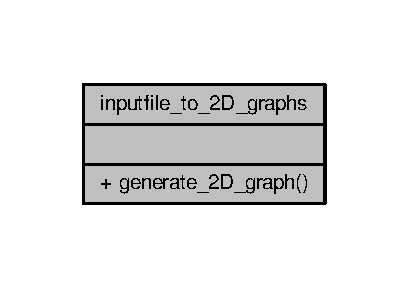
\includegraphics[width=196pt]{classinputfile__to__2D__graphs__coll__graph}
\end{center}
\end{figure}
\subsection*{Public Member Functions}
\begin{DoxyCompactItemize}
\item 
void \hyperlink{classinputfile__to__2D__graphs_af3d5444f4f09a556f66f6fbf9602aaa5}{generate\+\_\+2\+D\+\_\+graph} ()
\begin{DoxyCompactList}\small\item\em The input file will consist of 3 lists and each element of a list will consists of 2 co-\/ordinates having edges between them. \end{DoxyCompactList}\end{DoxyCompactItemize}


\subsection{Detailed Description}
An input file is converted into 3 2D graphs. 

\subsection{Member Function Documentation}
\index{inputfile\+\_\+to\+\_\+2\+D\+\_\+graphs@{inputfile\+\_\+to\+\_\+2\+D\+\_\+graphs}!generate\+\_\+2\+D\+\_\+graph@{generate\+\_\+2\+D\+\_\+graph}}
\index{generate\+\_\+2\+D\+\_\+graph@{generate\+\_\+2\+D\+\_\+graph}!inputfile\+\_\+to\+\_\+2\+D\+\_\+graphs@{inputfile\+\_\+to\+\_\+2\+D\+\_\+graphs}}
\subsubsection[{\texorpdfstring{generate\+\_\+2\+D\+\_\+graph()}{generate_2D_graph()}}]{\setlength{\rightskip}{0pt plus 5cm}void inputfile\+\_\+to\+\_\+2\+D\+\_\+graphs\+::generate\+\_\+2\+D\+\_\+graph (
\begin{DoxyParamCaption}
{}
\end{DoxyParamCaption}
)}\hypertarget{classinputfile__to__2D__graphs_af3d5444f4f09a556f66f6fbf9602aaa5}{}\label{classinputfile__to__2D__graphs_af3d5444f4f09a556f66f6fbf9602aaa5}


The input file will consist of 3 lists and each element of a list will consists of 2 co-\/ordinates having edges between them. 

The co-\/ordinates of the first list will be stored in the Vertex set of the first graph. The edges will be stored in the edge set after giving them weight according to the distance(which will be calculated) between 2 vertices. Similarly, the graphs for other lists will also be generated. The graphs generated will be objects \hyperlink{classgraph2D}{graph2D} class. \begin{DoxySeeAlso}{See also}
\hyperlink{classgraph2D}{graph2D} 
\end{DoxySeeAlso}


The documentation for this class was generated from the following file\+:\begin{DoxyCompactItemize}
\item 
\hyperlink{Canvas__2D_8cpp}{Canvas\+\_\+2\+D.\+cpp}\end{DoxyCompactItemize}

\hypertarget{classinputfile__to__3D__graph}{}\section{inputfile\+\_\+to\+\_\+3\+D\+\_\+graph Class Reference}
\label{classinputfile__to__3D__graph}\index{inputfile\+\_\+to\+\_\+3\+D\+\_\+graph@{inputfile\+\_\+to\+\_\+3\+D\+\_\+graph}}


An input file is converted to a 3D graph.  




Collaboration diagram for inputfile\+\_\+to\+\_\+3\+D\+\_\+graph\+:\nopagebreak
\begin{figure}[H]
\begin{center}
\leavevmode
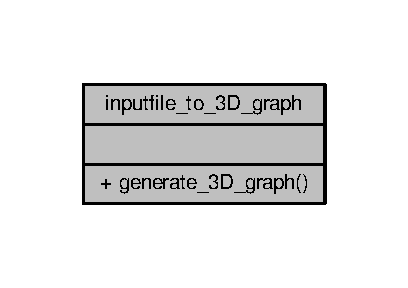
\includegraphics[width=196pt]{classinputfile__to__3D__graph__coll__graph}
\end{center}
\end{figure}
\subsection*{Public Member Functions}
\begin{DoxyCompactItemize}
\item 
\hyperlink{classgraph2D}{graph2D} \hyperlink{classinputfile__to__3D__graph_ab066fee3040885308398fa1033166a3b}{generate\+\_\+3\+D\+\_\+graph} ()
\begin{DoxyCompactList}\small\item\em The input file will consist of a list and each element of the list will consists of 2 co-\/ordinates having edges between them. \end{DoxyCompactList}\end{DoxyCompactItemize}


\subsection{Detailed Description}
An input file is converted to a 3D graph. 

\subsection{Member Function Documentation}
\index{inputfile\+\_\+to\+\_\+3\+D\+\_\+graph@{inputfile\+\_\+to\+\_\+3\+D\+\_\+graph}!generate\+\_\+3\+D\+\_\+graph@{generate\+\_\+3\+D\+\_\+graph}}
\index{generate\+\_\+3\+D\+\_\+graph@{generate\+\_\+3\+D\+\_\+graph}!inputfile\+\_\+to\+\_\+3\+D\+\_\+graph@{inputfile\+\_\+to\+\_\+3\+D\+\_\+graph}}
\subsubsection[{\texorpdfstring{generate\+\_\+3\+D\+\_\+graph()}{generate_3D_graph()}}]{\setlength{\rightskip}{0pt plus 5cm}{\bf graph2D} inputfile\+\_\+to\+\_\+3\+D\+\_\+graph\+::generate\+\_\+3\+D\+\_\+graph (
\begin{DoxyParamCaption}
{}
\end{DoxyParamCaption}
)}\hypertarget{classinputfile__to__3D__graph_ab066fee3040885308398fa1033166a3b}{}\label{classinputfile__to__3D__graph_ab066fee3040885308398fa1033166a3b}


The input file will consist of a list and each element of the list will consists of 2 co-\/ordinates having edges between them. 

The co-\/ordinates will be stored in the Vertex set of the graph. The edges will be stored in the edge set after giving them weight according to the distance(which will be calculated) between 2 vertices. The graph generated will be an object of \hyperlink{classgraph3D}{graph3D} class. \begin{DoxySeeAlso}{See also}
\hyperlink{classgraph3D}{graph3D} 
\end{DoxySeeAlso}


The documentation for this class was generated from the following file\+:\begin{DoxyCompactItemize}
\item 
\hyperlink{Canvas_8cpp}{Canvas.\+cpp}\end{DoxyCompactItemize}

\hypertarget{classmyvector}{}\section{myvector Class Reference}
\label{classmyvector}\index{myvector@{myvector}}


Collaboration diagram for myvector\+:\nopagebreak
\begin{figure}[H]
\begin{center}
\leavevmode
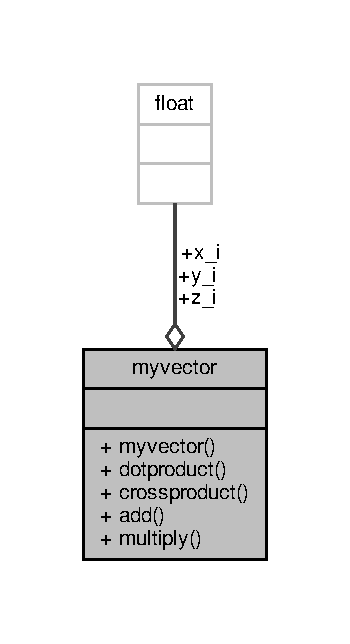
\includegraphics[width=168pt]{classmyvector__coll__graph}
\end{center}
\end{figure}
\subsection*{Public Member Functions}
\begin{DoxyCompactItemize}
\item 
\hyperlink{classmyvector_a50e56a1d0b5e3ba44c2cd87eb45cb7b4}{myvector} (int x, int y, int z)
\begin{DoxyCompactList}\small\item\em A Constructor. \end{DoxyCompactList}\item 
float \hyperlink{classmyvector_ab4164e997ce091642ba28a92b4db8cc6}{dotproduct} (\hyperlink{classmyvector}{myvector} p)
\begin{DoxyCompactList}\small\item\em A Member function which calculates dot product of two vectors. \end{DoxyCompactList}\item 
\hyperlink{classmyvector}{myvector} \hyperlink{classmyvector_af0caba3b74e0614eef1ccdff67372409}{crossproduct} (\hyperlink{classmyvector}{myvector} p)
\begin{DoxyCompactList}\small\item\em A Member function which calculates cross product of two vectors. \end{DoxyCompactList}\item 
\hyperlink{classmyvector}{myvector} \hyperlink{classmyvector_a2d07d77de689b075bbbe933a777197d1}{add} (\hyperlink{classmyvector}{myvector} p)
\item 
\hyperlink{classmyvector}{myvector} \hyperlink{classmyvector_a8eb11a1551c0ae3093f23cbd2a8b61fd}{multiply} (float n)
\end{DoxyCompactItemize}
\subsection*{Public Attributes}
\begin{DoxyCompactItemize}
\item 
float \hyperlink{classmyvector_ab893220476df8f4d0710871d02b76fe0}{x\+\_\+i}
\begin{DoxyCompactList}\small\item\em A public float member representing x-\/projection. \end{DoxyCompactList}\item 
float \hyperlink{classmyvector_ab61d4e74c6c20e28c93b23253c562889}{y\+\_\+i}
\begin{DoxyCompactList}\small\item\em A public float member representing y-\/projection. \end{DoxyCompactList}\item 
float \hyperlink{classmyvector_a1dcafb966fd664d2b6c633cd90f05216}{z\+\_\+i}
\begin{DoxyCompactList}\small\item\em A public float member representing z-\/projection. \end{DoxyCompactList}\end{DoxyCompactItemize}


\subsection{Constructor \& Destructor Documentation}
\index{myvector@{myvector}!myvector@{myvector}}
\index{myvector@{myvector}!myvector@{myvector}}
\subsubsection[{\texorpdfstring{myvector(int x, int y, int z)}{myvector(int x, int y, int z)}}]{\setlength{\rightskip}{0pt plus 5cm}myvector\+::myvector (
\begin{DoxyParamCaption}
\item[{int}]{x, }
\item[{int}]{y, }
\item[{int}]{z}
\end{DoxyParamCaption}
)}\hypertarget{classmyvector_a50e56a1d0b5e3ba44c2cd87eb45cb7b4}{}\label{classmyvector_a50e56a1d0b5e3ba44c2cd87eb45cb7b4}


A Constructor. 

The constructor initialies the vector. 
\begin{DoxyParams}{Parameters}
{\em x} & the x-\/projection. \\
\hline
{\em x} & the y-\/projection. \\
\hline
{\em x} & the z-\/projection. \\
\hline
\end{DoxyParams}


\subsection{Member Function Documentation}
\index{myvector@{myvector}!add@{add}}
\index{add@{add}!myvector@{myvector}}
\subsubsection[{\texorpdfstring{add(myvector p)}{add(myvector p)}}]{\setlength{\rightskip}{0pt plus 5cm}{\bf myvector} myvector\+::add (
\begin{DoxyParamCaption}
\item[{{\bf myvector}}]{p}
\end{DoxyParamCaption}
)}\hypertarget{classmyvector_a2d07d77de689b075bbbe933a777197d1}{}\label{classmyvector_a2d07d77de689b075bbbe933a777197d1}
\index{myvector@{myvector}!crossproduct@{crossproduct}}
\index{crossproduct@{crossproduct}!myvector@{myvector}}
\subsubsection[{\texorpdfstring{crossproduct(myvector p)}{crossproduct(myvector p)}}]{\setlength{\rightskip}{0pt plus 5cm}{\bf myvector} myvector\+::crossproduct (
\begin{DoxyParamCaption}
\item[{{\bf myvector}}]{p}
\end{DoxyParamCaption}
)}\hypertarget{classmyvector_af0caba3b74e0614eef1ccdff67372409}{}\label{classmyvector_af0caba3b74e0614eef1ccdff67372409}


A Member function which calculates cross product of two vectors. 

Calculates cross product of the object vector and the arguement vector and returns a new vector. 
\begin{DoxyParams}{Parameters}
{\em p} & A vector. \\
\hline
\end{DoxyParams}
\begin{DoxyReturn}{Returns}
The dot product(vector) 
\end{DoxyReturn}
\index{myvector@{myvector}!dotproduct@{dotproduct}}
\index{dotproduct@{dotproduct}!myvector@{myvector}}
\subsubsection[{\texorpdfstring{dotproduct(myvector p)}{dotproduct(myvector p)}}]{\setlength{\rightskip}{0pt plus 5cm}float myvector\+::dotproduct (
\begin{DoxyParamCaption}
\item[{{\bf myvector}}]{p}
\end{DoxyParamCaption}
)}\hypertarget{classmyvector_ab4164e997ce091642ba28a92b4db8cc6}{}\label{classmyvector_ab4164e997ce091642ba28a92b4db8cc6}


A Member function which calculates dot product of two vectors. 

Calculates dot product of the object vector and the arguement vector and returns a float value. 
\begin{DoxyParams}{Parameters}
{\em p} & A vector. \\
\hline
\end{DoxyParams}
\begin{DoxyReturn}{Returns}
The dot product(float value) 
\end{DoxyReturn}
\index{myvector@{myvector}!multiply@{multiply}}
\index{multiply@{multiply}!myvector@{myvector}}
\subsubsection[{\texorpdfstring{multiply(float n)}{multiply(float n)}}]{\setlength{\rightskip}{0pt plus 5cm}{\bf myvector} myvector\+::multiply (
\begin{DoxyParamCaption}
\item[{float}]{n}
\end{DoxyParamCaption}
)}\hypertarget{classmyvector_a8eb11a1551c0ae3093f23cbd2a8b61fd}{}\label{classmyvector_a8eb11a1551c0ae3093f23cbd2a8b61fd}


\subsection{Member Data Documentation}
\index{myvector@{myvector}!x\+\_\+i@{x\+\_\+i}}
\index{x\+\_\+i@{x\+\_\+i}!myvector@{myvector}}
\subsubsection[{\texorpdfstring{x\+\_\+i}{x_i}}]{\setlength{\rightskip}{0pt plus 5cm}float myvector\+::x\+\_\+i}\hypertarget{classmyvector_ab893220476df8f4d0710871d02b76fe0}{}\label{classmyvector_ab893220476df8f4d0710871d02b76fe0}


A public float member representing x-\/projection. 

\index{myvector@{myvector}!y\+\_\+i@{y\+\_\+i}}
\index{y\+\_\+i@{y\+\_\+i}!myvector@{myvector}}
\subsubsection[{\texorpdfstring{y\+\_\+i}{y_i}}]{\setlength{\rightskip}{0pt plus 5cm}float myvector\+::y\+\_\+i}\hypertarget{classmyvector_ab61d4e74c6c20e28c93b23253c562889}{}\label{classmyvector_ab61d4e74c6c20e28c93b23253c562889}


A public float member representing y-\/projection. 

\index{myvector@{myvector}!z\+\_\+i@{z\+\_\+i}}
\index{z\+\_\+i@{z\+\_\+i}!myvector@{myvector}}
\subsubsection[{\texorpdfstring{z\+\_\+i}{z_i}}]{\setlength{\rightskip}{0pt plus 5cm}float myvector\+::z\+\_\+i}\hypertarget{classmyvector_a1dcafb966fd664d2b6c633cd90f05216}{}\label{classmyvector_a1dcafb966fd664d2b6c633cd90f05216}


A public float member representing z-\/projection. 



The documentation for this class was generated from the following file\+:\begin{DoxyCompactItemize}
\item 
\hyperlink{main__computation_8cpp}{main\+\_\+computation.\+cpp}\end{DoxyCompactItemize}

\hypertarget{classoutput}{}\section{output Class Reference}
\label{classoutput}\index{output@{output}}


The output graphs are converted into a list and these lists are printed in an output file.  




Collaboration diagram for output\+:\nopagebreak
\begin{figure}[H]
\begin{center}
\leavevmode
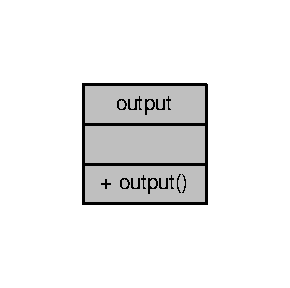
\includegraphics[width=139pt]{classoutput__coll__graph}
\end{center}
\end{figure}
\subsection*{Public Member Functions}
\begin{DoxyCompactItemize}
\item 
\hyperlink{classoutput_ad7e70fae10c1e8f527c0863ad69cab76}{output} ()
\begin{DoxyCompactList}\small\item\em A contructor The graphs are converted into a list. \end{DoxyCompactList}\end{DoxyCompactItemize}


\subsection{Detailed Description}
The output graphs are converted into a list and these lists are printed in an output file. 

\subsection{Constructor \& Destructor Documentation}
\index{output@{output}!output@{output}}
\index{output@{output}!output@{output}}
\subsubsection[{\texorpdfstring{output()}{output()}}]{\setlength{\rightskip}{0pt plus 5cm}output\+::output (
\begin{DoxyParamCaption}
{}
\end{DoxyParamCaption}
)}\hypertarget{classoutput_ad7e70fae10c1e8f527c0863ad69cab76}{}\label{classoutput_ad7e70fae10c1e8f527c0863ad69cab76}


A contructor The graphs are converted into a list. 

Firstly, the vertices having edge between them are identified. Then they are converted into a tuple and added to the list. This list is then stored into a file and the file is given as output to the user. 

The documentation for this class was generated from the following file\+:\begin{DoxyCompactItemize}
\item 
\hyperlink{Output_8cpp}{Output.\+cpp}\end{DoxyCompactItemize}

\hypertarget{classplane}{}\section{plane Class Reference}
\label{classplane}\index{plane@{plane}}


Class for a 3D plane.  




Collaboration diagram for plane\+:\nopagebreak
\begin{figure}[H]
\begin{center}
\leavevmode
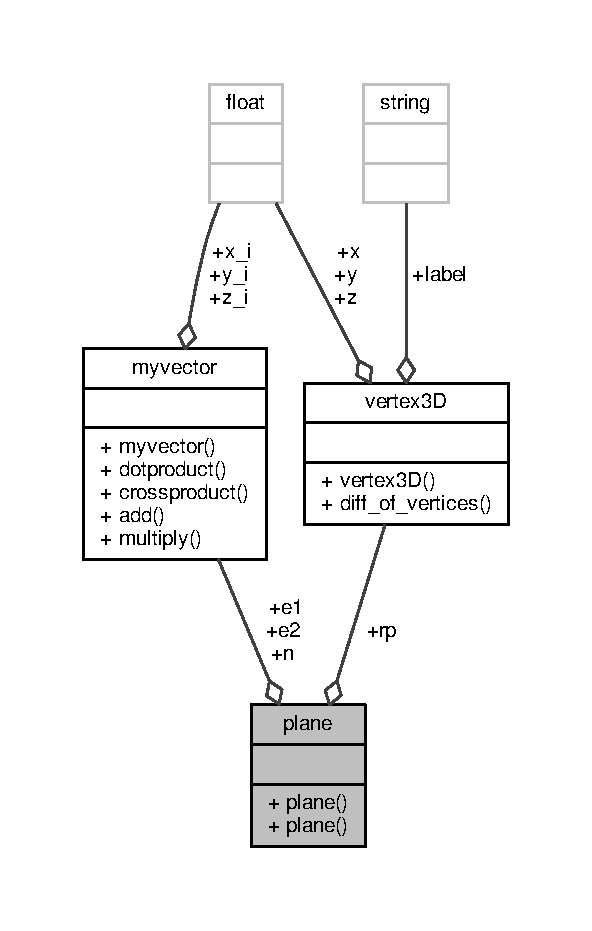
\includegraphics[width=284pt]{classplane__coll__graph}
\end{center}
\end{figure}
\subsection*{Public Member Functions}
\begin{DoxyCompactItemize}
\item 
\hyperlink{classplane_ab506ee0963b2469308760cad533b2539}{plane} (\hyperlink{classmyvector}{myvector} a, \hyperlink{classvertex3D}{vertex3D} $\ast$p, \hyperlink{classmyvector}{myvector} \hyperlink{classplane_a8edd6c4f34e5caae715c1f08b9898830}{e1})
\begin{DoxyCompactList}\small\item\em A Constructor. \end{DoxyCompactList}\item 
\hyperlink{classplane_a3f20707cf6b495058c537235a80c2ab8}{plane} (\hyperlink{classmyvector}{myvector} a, \hyperlink{classvertex3D}{vertex3D} $\ast$p)
\begin{DoxyCompactList}\small\item\em A Constructor. \end{DoxyCompactList}\end{DoxyCompactItemize}
\subsection*{Public Attributes}
\begin{DoxyCompactItemize}
\item 
\hyperlink{classmyvector}{myvector} \hyperlink{classplane_abb04a85adeef50a5fa72d150b3e1c2ce}{n}
\begin{DoxyCompactList}\small\item\em A public myvector object. \end{DoxyCompactList}\item 
\hyperlink{classmyvector}{myvector} \hyperlink{classplane_a8edd6c4f34e5caae715c1f08b9898830}{e1}
\begin{DoxyCompactList}\small\item\em A public myvector object. \end{DoxyCompactList}\item 
\hyperlink{classmyvector}{myvector} \hyperlink{classplane_aa642985b23f1d45bf21289bd71f4dc71}{e2}
\begin{DoxyCompactList}\small\item\em A public myvector object. \end{DoxyCompactList}\item 
\hyperlink{classvertex3D}{vertex3D} \hyperlink{classplane_ad2046f04a70e35c5803a1ebcfb678cf9}{rp}
\begin{DoxyCompactList}\small\item\em A public \hyperlink{classvertex3D}{vertex3D} object. \end{DoxyCompactList}\end{DoxyCompactItemize}


\subsection{Detailed Description}
Class for a 3D plane. 

Will be taken from the user. 

\subsection{Constructor \& Destructor Documentation}
\index{plane@{plane}!plane@{plane}}
\index{plane@{plane}!plane@{plane}}
\subsubsection[{\texorpdfstring{plane(myvector a, vertex3\+D $\ast$p, myvector e1)}{plane(myvector a, vertex3D *p, myvector e1)}}]{\setlength{\rightskip}{0pt plus 5cm}plane\+::plane (
\begin{DoxyParamCaption}
\item[{{\bf myvector}}]{a, }
\item[{{\bf vertex3D} $\ast$}]{p, }
\item[{{\bf myvector}}]{e1}
\end{DoxyParamCaption}
)}\hypertarget{classplane_ab506ee0963b2469308760cad533b2539}{}\label{classplane_ab506ee0963b2469308760cad533b2539}


A Constructor. 

The constructor has three arguements\+: a normal vector(n), point(rp), and one coordinate axis(e1). The other coordinate axis(e2) is calculated by crossproduct. 
\begin{DoxyParams}{Parameters}
{\em a} & the normal vector. \\
\hline
{\em p} & the point(3\+D vertex). \\
\hline
{\em e1} & the coordinate vector. \\
\hline
\end{DoxyParams}
\begin{DoxySeeAlso}{See also}
\hyperlink{classmyvector}{myvector} 

\hyperlink{classvertex3D}{vertex3D} 
\end{DoxySeeAlso}
\index{plane@{plane}!plane@{plane}}
\index{plane@{plane}!plane@{plane}}
\subsubsection[{\texorpdfstring{plane(myvector a, vertex3\+D $\ast$p)}{plane(myvector a, vertex3D *p)}}]{\setlength{\rightskip}{0pt plus 5cm}plane\+::plane (
\begin{DoxyParamCaption}
\item[{{\bf myvector}}]{a, }
\item[{{\bf vertex3D} $\ast$}]{p}
\end{DoxyParamCaption}
)}\hypertarget{classplane_a3f20707cf6b495058c537235a80c2ab8}{}\label{classplane_a3f20707cf6b495058c537235a80c2ab8}


A Constructor. 

The constructor has two arguements\+: a normal vector(n) and point(rp). e1 is intialized ourselves. The other coordinate axis(e2) is calculated by crossproduct. 
\begin{DoxyParams}{Parameters}
{\em a} & the normal vector. \\
\hline
{\em p} & the point(3\+D vertex). \\
\hline
\end{DoxyParams}
\begin{DoxySeeAlso}{See also}
\hyperlink{classmyvector}{myvector} 

\hyperlink{classvertex3D}{vertex3D} 
\end{DoxySeeAlso}


\subsection{Member Data Documentation}
\index{plane@{plane}!e1@{e1}}
\index{e1@{e1}!plane@{plane}}
\subsubsection[{\texorpdfstring{e1}{e1}}]{\setlength{\rightskip}{0pt plus 5cm}{\bf myvector} plane\+::e1}\hypertarget{classplane_a8edd6c4f34e5caae715c1f08b9898830}{}\label{classplane_a8edd6c4f34e5caae715c1f08b9898830}


A public myvector object. 

1st Coordinate axis along the plane. \begin{DoxySeeAlso}{See also}
\hyperlink{classmyvector}{myvector} 
\end{DoxySeeAlso}
\index{plane@{plane}!e2@{e2}}
\index{e2@{e2}!plane@{plane}}
\subsubsection[{\texorpdfstring{e2}{e2}}]{\setlength{\rightskip}{0pt plus 5cm}{\bf myvector} plane\+::e2}\hypertarget{classplane_aa642985b23f1d45bf21289bd71f4dc71}{}\label{classplane_aa642985b23f1d45bf21289bd71f4dc71}


A public myvector object. 

1st Coordinate axis along the plane. \begin{DoxySeeAlso}{See also}
\hyperlink{classmyvector}{myvector} 
\end{DoxySeeAlso}
\index{plane@{plane}!n@{n}}
\index{n@{n}!plane@{plane}}
\subsubsection[{\texorpdfstring{n}{n}}]{\setlength{\rightskip}{0pt plus 5cm}{\bf myvector} plane\+::n}\hypertarget{classplane_abb04a85adeef50a5fa72d150b3e1c2ce}{}\label{classplane_abb04a85adeef50a5fa72d150b3e1c2ce}


A public myvector object. 

Normal vector to the plane. \begin{DoxySeeAlso}{See also}
\hyperlink{classmyvector}{myvector} 
\end{DoxySeeAlso}
\index{plane@{plane}!rp@{rp}}
\index{rp@{rp}!plane@{plane}}
\subsubsection[{\texorpdfstring{rp}{rp}}]{\setlength{\rightskip}{0pt plus 5cm}{\bf vertex3D} plane\+::rp}\hypertarget{classplane_ad2046f04a70e35c5803a1ebcfb678cf9}{}\label{classplane_ad2046f04a70e35c5803a1ebcfb678cf9}


A public \hyperlink{classvertex3D}{vertex3D} object. 

A point on the plane. \begin{DoxySeeAlso}{See also}
\hyperlink{classvertex3D}{vertex3D} 
\end{DoxySeeAlso}


The documentation for this class was generated from the following file\+:\begin{DoxyCompactItemize}
\item 
\hyperlink{main__computation_8cpp}{main\+\_\+computation.\+cpp}\end{DoxyCompactItemize}

\hypertarget{classvertex2D}{}\section{vertex2D Class Reference}
\label{classvertex2D}\index{vertex2D@{vertex2D}}


Class for representing a 2D labelled vertex The vertex has a label and 2 coordinates.  


\subsection*{Public Member Functions}
\begin{DoxyCompactItemize}
\item 
\hyperlink{classvertex2D_a9f266c8c501d0349e35018d2ea66c56a}{vertex2D} (string name, float \hyperlink{classvertex2D_a2ba74d18c3e8e5a36fd2846a7a4d1a4f}{x}, float \hyperlink{classvertex2D_a6ca32b6427f8d3ce3437db0bafd92a00}{y})
\begin{DoxyCompactList}\small\item\em A Constructor. \end{DoxyCompactList}\item 
\hyperlink{classmyvector}{myvector} \hyperlink{classvertex2D_abf7a4ac8c177a3cc1b068a2df276a4cf}{diff\+\_\+of\+\_\+vertices} (\hyperlink{classvertex2D}{vertex2D} $\ast$v)
\begin{DoxyCompactList}\small\item\em A Member function which calculates the vector passing through two 2D vertices. \end{DoxyCompactList}\end{DoxyCompactItemize}
\subsection*{Public Attributes}
\begin{DoxyCompactItemize}
\item 
string \hyperlink{classvertex2D_a31103db4a64afce24d3d292f62ee3f3e}{label}
\begin{DoxyCompactList}\small\item\em A public string label denoting name of each vertex. \end{DoxyCompactList}\item 
float \hyperlink{classvertex2D_a2ba74d18c3e8e5a36fd2846a7a4d1a4f}{x}
\begin{DoxyCompactList}\small\item\em A public float member representing x-\/coordinate. \end{DoxyCompactList}\item 
float \hyperlink{classvertex2D_a6ca32b6427f8d3ce3437db0bafd92a00}{y}
\begin{DoxyCompactList}\small\item\em A public float member representing y-\/coordinate. \end{DoxyCompactList}\end{DoxyCompactItemize}


\subsection{Detailed Description}
Class for representing a 2D labelled vertex The vertex has a label and 2 coordinates. 

Used in constructing 2D graph. 

\subsection{Constructor \& Destructor Documentation}
\index{vertex2D@{vertex2D}!vertex2D@{vertex2D}}
\index{vertex2D@{vertex2D}!vertex2D@{vertex2D}}
\subsubsection[{\texorpdfstring{vertex2\+D(string name, float x, float y)}{vertex2D(string name, float x, float y)}}]{\setlength{\rightskip}{0pt plus 5cm}vertex2\+D\+::vertex2D (
\begin{DoxyParamCaption}
\item[{string}]{name, }
\item[{float}]{x, }
\item[{float}]{y}
\end{DoxyParamCaption}
)}\hypertarget{classvertex2D_a9f266c8c501d0349e35018d2ea66c56a}{}\label{classvertex2D_a9f266c8c501d0349e35018d2ea66c56a}


A Constructor. 

The constructor which initialies the 2D vertex. 
\begin{DoxyParams}{Parameters}
{\em name} & the label. \\
\hline
{\em x} & the x-\/coordinate. \\
\hline
{\em y} & the y-\/coordinate. \\
\hline
\end{DoxyParams}


\subsection{Member Function Documentation}
\index{vertex2D@{vertex2D}!diff\+\_\+of\+\_\+vertices@{diff\+\_\+of\+\_\+vertices}}
\index{diff\+\_\+of\+\_\+vertices@{diff\+\_\+of\+\_\+vertices}!vertex2D@{vertex2D}}
\subsubsection[{\texorpdfstring{diff\+\_\+of\+\_\+vertices(vertex2\+D $\ast$v)}{diff_of_vertices(vertex2D *v)}}]{\setlength{\rightskip}{0pt plus 5cm}{\bf myvector} vertex2\+D\+::diff\+\_\+of\+\_\+vertices (
\begin{DoxyParamCaption}
\item[{{\bf vertex2D} $\ast$}]{v}
\end{DoxyParamCaption}
)}\hypertarget{classvertex2D_abf7a4ac8c177a3cc1b068a2df276a4cf}{}\label{classvertex2D_abf7a4ac8c177a3cc1b068a2df276a4cf}


A Member function which calculates the vector passing through two 2D vertices. 

Calculates difference of the object vertex and the arguement vertex and returns a new vector. 
\begin{DoxyParams}{Parameters}
{\em p} & A 2D vertex. \\
\hline
\end{DoxyParams}
\begin{DoxyReturn}{Returns}
The vector 
\end{DoxyReturn}


\subsection{Member Data Documentation}
\index{vertex2D@{vertex2D}!label@{label}}
\index{label@{label}!vertex2D@{vertex2D}}
\subsubsection[{\texorpdfstring{label}{label}}]{\setlength{\rightskip}{0pt plus 5cm}string vertex2\+D\+::label}\hypertarget{classvertex2D_a31103db4a64afce24d3d292f62ee3f3e}{}\label{classvertex2D_a31103db4a64afce24d3d292f62ee3f3e}


A public string label denoting name of each vertex. 

\index{vertex2D@{vertex2D}!x@{x}}
\index{x@{x}!vertex2D@{vertex2D}}
\subsubsection[{\texorpdfstring{x}{x}}]{\setlength{\rightskip}{0pt plus 5cm}float vertex2\+D\+::x}\hypertarget{classvertex2D_a2ba74d18c3e8e5a36fd2846a7a4d1a4f}{}\label{classvertex2D_a2ba74d18c3e8e5a36fd2846a7a4d1a4f}


A public float member representing x-\/coordinate. 

\index{vertex2D@{vertex2D}!y@{y}}
\index{y@{y}!vertex2D@{vertex2D}}
\subsubsection[{\texorpdfstring{y}{y}}]{\setlength{\rightskip}{0pt plus 5cm}float vertex2\+D\+::y}\hypertarget{classvertex2D_a6ca32b6427f8d3ce3437db0bafd92a00}{}\label{classvertex2D_a6ca32b6427f8d3ce3437db0bafd92a00}


A public float member representing y-\/coordinate. 



The documentation for this class was generated from the following file\+:\begin{DoxyCompactItemize}
\item 
\hyperlink{main__computation_8cpp}{main\+\_\+computation.\+cpp}\end{DoxyCompactItemize}

\hypertarget{classvertex3D}{}\section{vertex3D Class Reference}
\label{classvertex3D}\index{vertex3D@{vertex3D}}


Class for representing a 3D labelled vertex The vertex has a label and 3 coordinates.  




Collaboration diagram for vertex3D\+:\nopagebreak
\begin{figure}[H]
\begin{center}
\leavevmode
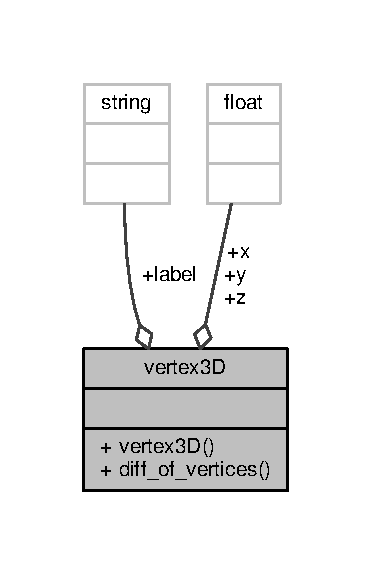
\includegraphics[width=178pt]{classvertex3D__coll__graph}
\end{center}
\end{figure}
\subsection*{Public Member Functions}
\begin{DoxyCompactItemize}
\item 
\hyperlink{classvertex3D_a82301ce369a5bff49f467f73b93e3d67}{vertex3D} (string name, float \hyperlink{classvertex3D_a6c6ee4315d72adbc5abb17e6af802087}{x}, float \hyperlink{classvertex3D_aa1f4823bf2a3f648b1b0b39ef7ea5891}{y}, float \hyperlink{classvertex3D_a67f3819dff895cb47284c34ec85658d7}{z})
\begin{DoxyCompactList}\small\item\em A Constructor. \end{DoxyCompactList}\item 
\hyperlink{classmyvector}{myvector} \hyperlink{classvertex3D_aaf451bdb095243ff34d788648aa8ff29}{diff\+\_\+of\+\_\+vertices} (\hyperlink{classvertex3D}{vertex3D} $\ast$v)
\begin{DoxyCompactList}\small\item\em A Member function which calculates the vector passing through two 3D vertices. \end{DoxyCompactList}\end{DoxyCompactItemize}
\subsection*{Public Attributes}
\begin{DoxyCompactItemize}
\item 
string \hyperlink{classvertex3D_a4c67b08d630abdaae2fc2816002753a7}{label}
\begin{DoxyCompactList}\small\item\em A public string label denoting name of each vertex. \end{DoxyCompactList}\item 
float \hyperlink{classvertex3D_a6c6ee4315d72adbc5abb17e6af802087}{x}
\begin{DoxyCompactList}\small\item\em A public float member representing x-\/coordinate. \end{DoxyCompactList}\item 
float \hyperlink{classvertex3D_aa1f4823bf2a3f648b1b0b39ef7ea5891}{y}
\begin{DoxyCompactList}\small\item\em A public float member representing y-\/coordinate. \end{DoxyCompactList}\item 
float \hyperlink{classvertex3D_a67f3819dff895cb47284c34ec85658d7}{z}
\begin{DoxyCompactList}\small\item\em A public float member representing z-\/coordinate. \end{DoxyCompactList}\end{DoxyCompactItemize}


\subsection{Detailed Description}
Class for representing a 3D labelled vertex The vertex has a label and 3 coordinates. 

Used in constructing 3D graph. 

\subsection{Constructor \& Destructor Documentation}
\index{vertex3D@{vertex3D}!vertex3D@{vertex3D}}
\index{vertex3D@{vertex3D}!vertex3D@{vertex3D}}
\subsubsection[{\texorpdfstring{vertex3\+D(string name, float x, float y, float z)}{vertex3D(string name, float x, float y, float z)}}]{\setlength{\rightskip}{0pt plus 5cm}vertex3\+D\+::vertex3D (
\begin{DoxyParamCaption}
\item[{string}]{name, }
\item[{float}]{x, }
\item[{float}]{y, }
\item[{float}]{z}
\end{DoxyParamCaption}
)}\hypertarget{classvertex3D_a82301ce369a5bff49f467f73b93e3d67}{}\label{classvertex3D_a82301ce369a5bff49f467f73b93e3d67}


A Constructor. 

The constructor which initialies the 3D vertex. 
\begin{DoxyParams}{Parameters}
{\em name} & the label. \\
\hline
{\em x} & the x-\/coordinate. \\
\hline
{\em y} & the y-\/coordinate. \\
\hline
{\em z} & the z-\/coordinate. \\
\hline
\end{DoxyParams}


\subsection{Member Function Documentation}
\index{vertex3D@{vertex3D}!diff\+\_\+of\+\_\+vertices@{diff\+\_\+of\+\_\+vertices}}
\index{diff\+\_\+of\+\_\+vertices@{diff\+\_\+of\+\_\+vertices}!vertex3D@{vertex3D}}
\subsubsection[{\texorpdfstring{diff\+\_\+of\+\_\+vertices(vertex3\+D $\ast$v)}{diff_of_vertices(vertex3D *v)}}]{\setlength{\rightskip}{0pt plus 5cm}{\bf myvector} vertex3\+D\+::diff\+\_\+of\+\_\+vertices (
\begin{DoxyParamCaption}
\item[{{\bf vertex3D} $\ast$}]{v}
\end{DoxyParamCaption}
)}\hypertarget{classvertex3D_aaf451bdb095243ff34d788648aa8ff29}{}\label{classvertex3D_aaf451bdb095243ff34d788648aa8ff29}


A Member function which calculates the vector passing through two 3D vertices. 

Calculates difference of the object vertex and the arguement vertex and returns a new vector. 
\begin{DoxyParams}{Parameters}
{\em p} & A 3D vertex. \\
\hline
\end{DoxyParams}
\begin{DoxyReturn}{Returns}
The vector 
\end{DoxyReturn}


\subsection{Member Data Documentation}
\index{vertex3D@{vertex3D}!label@{label}}
\index{label@{label}!vertex3D@{vertex3D}}
\subsubsection[{\texorpdfstring{label}{label}}]{\setlength{\rightskip}{0pt plus 5cm}string vertex3\+D\+::label}\hypertarget{classvertex3D_a4c67b08d630abdaae2fc2816002753a7}{}\label{classvertex3D_a4c67b08d630abdaae2fc2816002753a7}


A public string label denoting name of each vertex. 

\index{vertex3D@{vertex3D}!x@{x}}
\index{x@{x}!vertex3D@{vertex3D}}
\subsubsection[{\texorpdfstring{x}{x}}]{\setlength{\rightskip}{0pt plus 5cm}float vertex3\+D\+::x}\hypertarget{classvertex3D_a6c6ee4315d72adbc5abb17e6af802087}{}\label{classvertex3D_a6c6ee4315d72adbc5abb17e6af802087}


A public float member representing x-\/coordinate. 

\index{vertex3D@{vertex3D}!y@{y}}
\index{y@{y}!vertex3D@{vertex3D}}
\subsubsection[{\texorpdfstring{y}{y}}]{\setlength{\rightskip}{0pt plus 5cm}float vertex3\+D\+::y}\hypertarget{classvertex3D_aa1f4823bf2a3f648b1b0b39ef7ea5891}{}\label{classvertex3D_aa1f4823bf2a3f648b1b0b39ef7ea5891}


A public float member representing y-\/coordinate. 

\index{vertex3D@{vertex3D}!z@{z}}
\index{z@{z}!vertex3D@{vertex3D}}
\subsubsection[{\texorpdfstring{z}{z}}]{\setlength{\rightskip}{0pt plus 5cm}float vertex3\+D\+::z}\hypertarget{classvertex3D_a67f3819dff895cb47284c34ec85658d7}{}\label{classvertex3D_a67f3819dff895cb47284c34ec85658d7}


A public float member representing z-\/coordinate. 



The documentation for this class was generated from the following file\+:\begin{DoxyCompactItemize}
\item 
\hyperlink{main__computation_8cpp}{main\+\_\+computation.\+cpp}\end{DoxyCompactItemize}

\chapter{File Documentation}
\hypertarget{Canvas_8cpp}{}\section{Canvas.\+cpp File Reference}
\label{Canvas_8cpp}\index{Canvas.\+cpp@{Canvas.\+cpp}}
{\ttfamily \#include $<$bits/stdc++.\+h$>$}\\*
{\ttfamily \#include $<$main\+\_\+computation.\+cpp$>$}\\*
Include dependency graph for Canvas.\+cpp\+:
\nopagebreak
\begin{figure}[H]
\begin{center}
\leavevmode
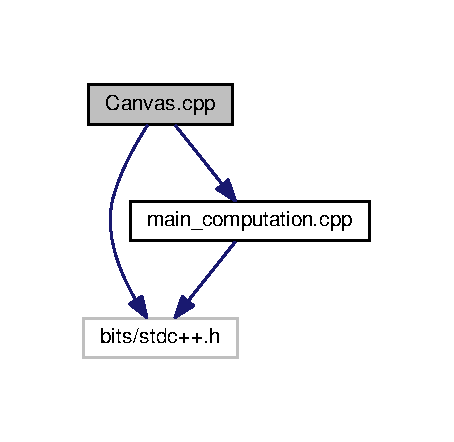
\includegraphics[width=218pt]{Canvas_8cpp__incl}
\end{center}
\end{figure}
This graph shows which files directly or indirectly include this file\+:
\nopagebreak
\begin{figure}[H]
\begin{center}
\leavevmode
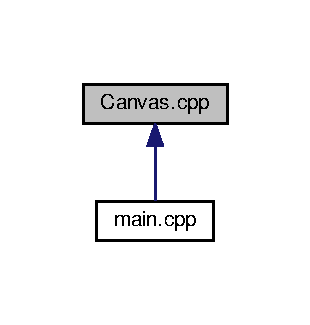
\includegraphics[width=149pt]{Canvas_8cpp__dep__incl}
\end{center}
\end{figure}
\subsection*{Classes}
\begin{DoxyCompactItemize}
\item 
class \hyperlink{classinputfile__to__2D__graphs}{inputfile\+\_\+to\+\_\+2\+D\+\_\+graphs}
\begin{DoxyCompactList}\small\item\em An input file is converted into 3 2D graphs. \end{DoxyCompactList}\item 
class \hyperlink{classinputfile__to__3D__graph}{inputfile\+\_\+to\+\_\+3\+D\+\_\+graph}
\begin{DoxyCompactList}\small\item\em An input file is converted to a 3D graph. \end{DoxyCompactList}\end{DoxyCompactItemize}

\hypertarget{Input__mode_8cpp}{}\section{Input\+\_\+mode.\+cpp File Reference}
\label{Input__mode_8cpp}\index{Input\+\_\+mode.\+cpp@{Input\+\_\+mode.\+cpp}}
{\ttfamily \#include $<$bits/stdc++.\+h$>$}\\*
Include dependency graph for Input\+\_\+mode.\+cpp\+:\nopagebreak
\begin{figure}[H]
\begin{center}
\leavevmode
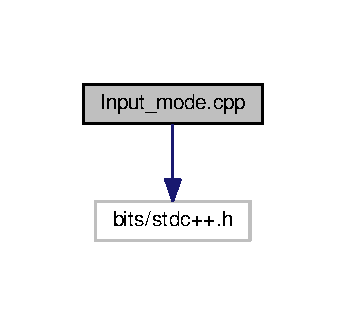
\includegraphics[width=166pt]{Input__mode_8cpp__incl}
\end{center}
\end{figure}
This graph shows which files directly or indirectly include this file\+:
\nopagebreak
\begin{figure}[H]
\begin{center}
\leavevmode
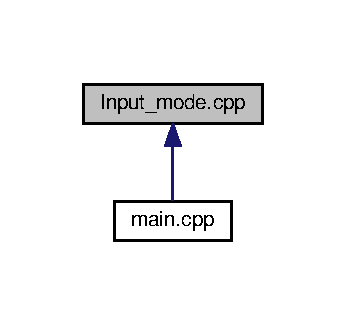
\includegraphics[width=166pt]{Input__mode_8cpp__dep__incl}
\end{center}
\end{figure}
\subsection*{Classes}
\begin{DoxyCompactItemize}
\item 
class \hyperlink{classinput__mode}{input\+\_\+mode}
\begin{DoxyCompactList}\small\item\em User Mode selection is done here. \end{DoxyCompactList}\end{DoxyCompactItemize}

\hypertarget{main_8cpp}{}\section{main.\+cpp File Reference}
\label{main_8cpp}\index{main.\+cpp@{main.\+cpp}}
{\ttfamily \#include $<$bits/stdc++.\+h$>$}\\*
Include dependency graph for main.\+cpp\+:
% FIG 0
\subsection*{Functions}
\begin{DoxyCompactItemize}
\item 
int \hyperlink{main_8cpp_ae66f6b31b5ad750f1fe042a706a4e3d4}{main} ()
\begin{DoxyCompactList}\small\item\em The main function. \end{DoxyCompactList}\end{DoxyCompactItemize}


\subsection{Function Documentation}
\index{main.\+cpp@{main.\+cpp}!main@{main}}
\index{main@{main}!main.\+cpp@{main.\+cpp}}
\subsubsection[{\texorpdfstring{main()}{main()}}]{\setlength{\rightskip}{0pt plus 5cm}int main (
\begin{DoxyParamCaption}
{}
\end{DoxyParamCaption}
)}\hypertarget{main_8cpp_ae66f6b31b5ad750f1fe042a706a4e3d4}{}\label{main_8cpp_ae66f6b31b5ad750f1fe042a706a4e3d4}


The main function. 

Does all the operations by making objects and calling respective functions. Checks input mode, then takes desired input, converts to graph. Then graph interconversion takes place i.\+e 2D to 3D or 3D to 2D. Gives the output. See the below classes for respective details. \begin{DoxySeeAlso}{See also}
\hyperlink{classinput__mode}{input\+\_\+mode} 

\hyperlink{classinputfile__to__2D__graphs}{inputfile\+\_\+to\+\_\+2\+D\+\_\+graphs} 

\hyperlink{classinputfile__to__3D__graph}{inputfile\+\_\+to\+\_\+3\+D\+\_\+graph} 

\hyperlink{classoutput}{output} 
\end{DoxySeeAlso}

\hypertarget{main__computation_8cpp}{}\section{main\+\_\+computation.\+cpp File Reference}
\label{main__computation_8cpp}\index{main\+\_\+computation.\+cpp@{main\+\_\+computation.\+cpp}}
{\ttfamily \#include $<$bits/stdc++.\+h$>$}\\*
Include dependency graph for main\+\_\+computation.\+cpp\+:\nopagebreak
\begin{figure}[H]
\begin{center}
\leavevmode
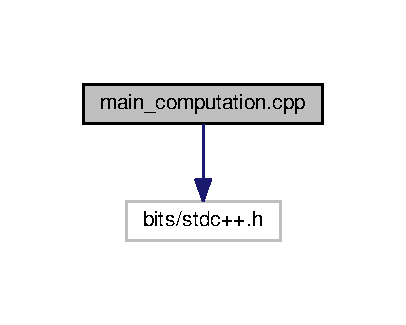
\includegraphics[width=195pt]{main__computation_8cpp__incl}
\end{center}
\end{figure}
This graph shows which files directly or indirectly include this file\+:
\nopagebreak
\begin{figure}[H]
\begin{center}
\leavevmode
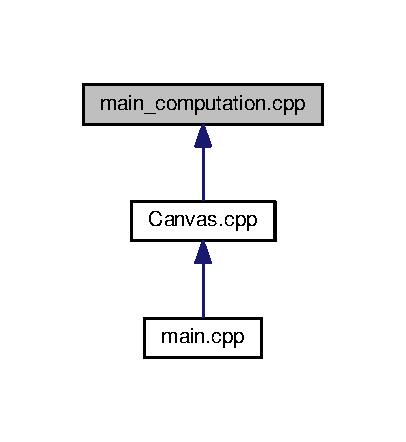
\includegraphics[width=195pt]{main__computation_8cpp__dep__incl}
\end{center}
\end{figure}
\subsection*{Classes}
\begin{DoxyCompactItemize}
\item 
class \hyperlink{classmyvector}{myvector}
\item 
class \hyperlink{classvertex3D}{vertex3D}
\begin{DoxyCompactList}\small\item\em Class for representing a 3D labelled vertex The vertex has a label and 3 coordinates. \end{DoxyCompactList}\item 
class \hyperlink{classvertex2D}{vertex2D}
\begin{DoxyCompactList}\small\item\em Class for representing a 2D labelled vertex The vertex has a label and 2 coordinates. \end{DoxyCompactList}\item 
class \hyperlink{classplane}{plane}
\begin{DoxyCompactList}\small\item\em Class for a 3D plane. \end{DoxyCompactList}\item 
class \hyperlink{classgraph3D}{graph3D}
\begin{DoxyCompactList}\small\item\em Class for 3D graph. \end{DoxyCompactList}\item 
class \hyperlink{classgraph2D}{graph2D}
\begin{DoxyCompactList}\small\item\em Class for 2D graph. \end{DoxyCompactList}\end{DoxyCompactItemize}

\hypertarget{Output_8cpp}{}\section{Output.\+cpp File Reference}
\label{Output_8cpp}\index{Output.\+cpp@{Output.\+cpp}}
{\ttfamily \#include $<$bits/stdc++.\+h$>$}\\*
{\ttfamily \#include $<$main\+\_\+computation.\+cpp$>$}\\*
{\ttfamily \#include $<$Canvas\+\_\+3\+D.\+cpp$>$}\\*
{\ttfamily \#include $<$Canvas\+\_\+2\+D.\+cpp$>$}\\*
Include dependency graph for Output.\+cpp\+:\nopagebreak
\begin{figure}[H]
\begin{center}
\leavevmode
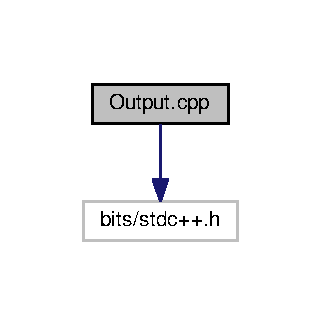
\includegraphics[width=350pt]{Output_8cpp__incl}
\end{center}
\end{figure}
This graph shows which files directly or indirectly include this file\+:\nopagebreak
\begin{figure}[H]
\begin{center}
\leavevmode
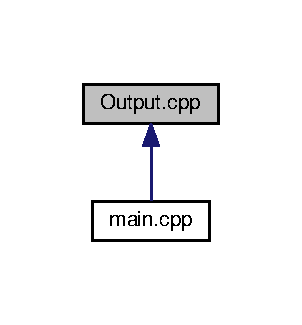
\includegraphics[width=145pt]{Output_8cpp__dep__incl}
\end{center}
\end{figure}
\subsection*{Classes}
\begin{DoxyCompactItemize}
\item 
class \hyperlink{classoutput}{output}
\begin{DoxyCompactList}\small\item\em The output graphs are converted into a list and these lists are printed in an output file. \end{DoxyCompactList}\end{DoxyCompactItemize}

%--- End generated contents ---

% Index
\backmatter
\newpage
\phantomsection
\clearemptydoublepage
\addcontentsline{toc}{chapter}{Index}
\printindex

\end{document}
